\subsection{Quantifying Goodhart's law}

Our work is concerned with \emph{quantifying} the Goodhart effect. To do this, we need a way to quantify the \emph{distance between rewards}. We do this using the \emph{projected angle between reward vectors}.

\begin{definition}[Projected angle]\label{def:angle-distance}
    Given two reward functions $\TrueR, \ProxR$, we define $\Angle{\TrueR}{\ProxR}$ to be the angle between $\QProj_\T \TrueR$ and $\QProj_\T \ProxR$.
\end{definition}

The projected angle distance is an instance of a \emph{STARC metric}, introduced by \citet{skalse2023starc}.\footnote{In their terminology, the \emph{canonicalisation function} is $\QProj_\T$, and measuring the angle between the resulting vectors is (bilipschitz) equivalent to normalising and measuring the distance with the $\ell^2$-norm.} Such metrics enjoy strong theoretical guarantees and satisfy many desirable desiderata for reward function metrics. For details, see \citet{skalse2023starc}. In particular:

\begin{proposition}
We have $\Angle{\TrueR}{\ProxR} = 0$ if and only if $\TrueR, \ProxR$ induce the same ordering of policies, or, in other words, $\J_{\TrueR}(\policy) \leq \J_{\TrueR}(\policy') \iff \J_{\ProxR}(\policy) \leq \J_{\ProxR}(\policy')$ for all policies $\policy, \policy'$.
\end{proposition}

We also need a way to quantify \emph{optimisation pressure}. We do this using two different training methods. Both are parametrised by \emph{regularisation strength} $\alpha \in (0, \infty)$: Given a reward $\R$, they output a regularised policy $\policy_\alpha$. 
For ease of discussion and plotting, it is often more appropriate to refer to the (bounded) inverse of the regularisation strength: the \emph{optimisation pressure} $\lambda_\alpha = e^{-\alpha}$. As the optimisation pressure increases, $\J(\policy_\alpha)$ also increases.

\begin{definition}[Maximal Causal Entropy]\label{def:mce}
    We denote by $\pi_{\alpha}$ the optimal policy according to the regularised objective $\tilde{\R}(s, a) := \R(s, a) +\alpha H(\pi(s))$ where $H(\pi(s))$ is the Shannon entropy.
\end{definition}

\begin{definition}[Boltzmann Rationality]\label{def:br}
    The Boltzmann rational policy $\policy_\alpha$ is defined as $\Prob{\policy_\alpha(s) = a} \propto e^{\frac{1}{\alpha} Q^\star(s, a)}$, where $Q^\star$ is the optimal $Q$-function.
\end{definition}


We perform experiments to verify that our key results hold for either way of quantifying optimisation pressure. In both cases, the optimisation algorithm is Value Iteration \citep[see e.g.\ ][]{sutton2018}.


Finally, we need a way to quantify the \emph{magnitude of the Goodhart effect}. Assume that we have a true reward $R_0$ and a proxy reward $R_1$, that $R_1$ is optimised according to one of the methods in Definition~\ref{def:mce}-\ref{def:br}, and that $\pi_\lambda$ is the policy that is obtained at optimisation pressure $\lambda$. Suppose also that $R_0, R_1$ are normalised, so that $\min_\pi \J(\pi) = 0$ and $\max_\pi \J(\pi) = 1$ for both $R_0$ and $R_1$.


\begin{definition}[Normalised drop height]
We define the \emph{normalised drop height} (NDH) as $\J_{\TrueR}(\pi_1) - \max_{\lambda \in [0,1]} \J_{\TrueR}(\pi_\lambda)$, i.e.\ as the loss of true reward throughout the optimisation process.
\end{definition}
For an illustration of the above definition, see the grey dashed line in~\Cref{fig:goodhart_cartoon}. We observe that NDH is non-zero if and only if, over increasing optimisation pressure, the proxy and true rewards are initially correlated, and then become anti-correlated (we will see later that as long as the angle distance is less than $\pi/2$, their returns will almost always be initially correlated)\jacek{Rephrase this sentence about $<\pi/2$}. In the Appendix~\ref{appendix:measuring_goodharting}, we introduce more complex measures which quantify Goodhart's law differently. Since our experiments indicate that they are all are strongly correlated, we decided to focus on NDH as the simplest one.

\section{Goodharting is Pervasive in Reinforcement Learning}\label{sec:quantifying_goodharting}

\begin{figure}
    \centering
    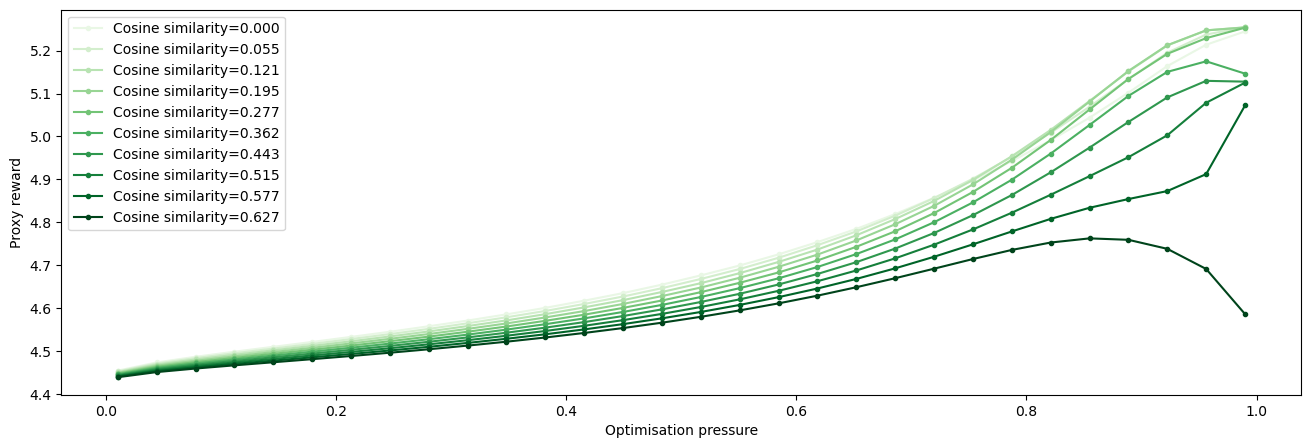
\includegraphics[width=0.78\linewidth]{goodharting_happens/RandomMDP_plot.png}
    \caption{Depiction of Goodharting in \emph{RandomMDP}. 
    Compare to~\Cref{fig:goodhart_cartoon} -- here we only show the \emph{true} reward obtained by a policy trained on each proxy. Darker color means a more distant proxy.\label{fig:RandomMDP}
    }
\end{figure}

In this section, we empirically demonstrate that Goodharting occurs pervasively across varied environments by showing that, for a given true reward $\TrueR$ and a proxy reward $\ProxR$, beyond a certain optimisation threshold, the performance on $\TrueR$ \emph{decreases} when the agent is trained towards $\ProxR$. We test this claim over different kinds of environments (varying number of states, actions, terminal states and $\gamma$), reward functions (varying rewards' types and sparsity) and optimisation pressure definitions.

\subsection{Environment and reward types}

\emph{Gridworld} is a deterministic, grid-based environment, with the state space of size $n \times n$ for parameter $n \in \mathbb{N}^+$, with a fixed set of five actions: $\uparrow, \rightarrow, \downarrow, \leftarrow$, and \text{WAIT}. The upper-left and lower-right corners are designated as terminal states. Attempting an illegal action $a$ in state $s$ does not change the state. \emph{Cliff}~\citep[Example 6.6]{sutton2018} is a \emph{Gridworld} variant where an agent aims to reach the lower right terminal state, avoiding the cliff formed by the bottom row's cells. Any cliff-adjacent move has a slipping probability $p$ of falling into the cliff.

\emph{RandomMDP} is an environment in which, for a fixed number of states $|S|$, actions $|A|$, and terminal states $k$, the transition matrix $\T$ is sampled uniformly across all stochastic matrices of shape $|\SxA|\times |S|$, satisfying the property of having exactly $k$ terminal states.

\emph{TreeMDP} is an environment corresponding to nodes of a rooted tree with branching factor $b = |\A|$ and depth $d$. The root is the initial state and each action from a non-leaf node results in states corresponding to the node's children. Half of the leaf nodes are terminal states and the other half loop back to the root, which makes it isomorphic to an infinite self-similar tree.

In our experiments, we only use reward functions that depend on the next state $R(s, a) = R(s)$. In \textbf{Terminal}, the rewards are sampled iid from $U(0, 1)$ for terminal states and from $U(-1, 0)$ for non-terminal states. In \textbf{Cliff}, where the rewards are sampled iid from $U(-5, 0)$ for cliff states, from $U(-1, 0)$ for non-terminal states, and from $U(0, 1)$ for the goal state. In \textbf{Path}, where we first sample a random walk $P$ moving only $\rightarrow$ and $\downarrow$ between the upper-left and lower-right terminal state, and then the rewards are constantly 0 on the path $P$, sampled from $U(-1, 0)$ for the non-terminal states, and from $U(0, 1)$ for the terminal state.

\subsection{Estimating the prevalence of Goodharting}\label{subsect:estimating-prevalence}

To get an estimate of how prevalent Goodharting is, we run an experiment where we vary all hyperparameters of MDPs in a grid search manner. Specifically, we sample:
\emph{Gridworld} for grid lengths $n \in \{2, 3, \dots, 14\}$ %$n \in \{2, 3, 4, 5, 6, 7, 8, 9, 10, 11, 12, 13, 14\}$ 
and either \textbf{Terminal} or \textbf{Path} rewards;
\emph{Cliff} with tripping probability $p = 0.5$ and grid lengths $n \in \{2, 3, \dots, 9\}$ %$n \in \{2, 3, 4, 5, 6, 7, 8, 9\}$ 
and \textbf{Cliff} rewards; 
\emph{RandomMDP} with number of states $|S| \in \{2, 4, 8, 16, \dots, 512\}$, %$|S| \in \{2, 4, 8, 16, 32, 64, 128, 256, 512\}$,
number of actions $|A| \in \{2, 3, 4\}$, a fixed number of terminal states $=2$, and \textbf{Terminal} rewards;
\emph{TreeMDP} with branching factor $2$ and depth $d \in [2, 3, \dots, 9]$, %$d \in [2, 3, 4, 5, 6, 7, 8, 9]$, 
for two different kinds of trees: (1) where the first half of the leaves are terminal states, and (2) where every second leaf is a terminal state, both using \textbf{Terminal} rewards.

For each of those, we also vary temporal discount factor $\gamma \in \{0.5, 0.7, 0.9, 0.99\}$, sparsity factor $\sigma \in \{0.1, 0.3, 0.5, 0.7, 0.9\}$, optimisation pressure $\lambda = -\log(x)$ for $7$ values of $x$ evenly spaced on $[0.01, 0.75]$ and $20$ values evenly spaced on $[0.8, 0.99]$.

After sampling an MDP\textbackslash R, we randomly sample a pair of reward functions $\R_0$ and $\R_1$ from a chosen distribution. These are then sparsified (meaning that a random $\sigma$ fraction of values are zeroed) and linearly interpolated, creating a sequence of proxy reward functions $\R_t = (1-t)\R_0 + t\R_1$ for $t \in [0,1]$. 
Note that this scheme is valid because for any environment, reward sampling scheme and fixed parameters, the sample space of rewards is convex. In high dimensions, two random vectors are approximately orthogonal with high probability, so the sequence $R_t$ spans a range of distances.

Each run consists of $10$ proxy rewards; we use threshold $\theta = 0.001$ for value iteration. We get a total of 30400 data points. An initial increase, followed by a decline in value with increasing optimisation pressure, indicates Goodharting behaviour. Overall, we find that a Goodhart drop occurs (meaning that the NDH > 0) for \textbf{19.3\% of all experiments} sampled over the parameter ranges given above. This suggests that Goodharting is a common (albeit not universal) phenomenon in RL and occurs in various environments and for various reward functions. We present additional empirical insights, such as that training \emph{myopic} agents makes  Goodharting less severe, in \Cref{appendix: results}.

For illustrative purposes, we present a single run of the above experiment in ~\Cref{fig:RandomMDP}. We can see that, as the proxy $\ProxR$ is maximised, the true reward $\TrueR$ will typically either increase monotonically or increase and then decrease. This is in accordance with the predictions of Goodhart's law.

